\section{Introduction}

For autonomous robots and unmanned vehicles to execute their tasks effectively, they require: accurate self-location information, and detailed maps of the environment.
However, these requirements aren't always feasible or dependable due to the following reasons:
\begin{itemize}
    \item Global Navigation Satellite Systems (GNSS) may not always be reliable or available.
    \item Not all areas have been accurately mapped.
    \item Environmental conditions can change dynamically.
    \item Maps need regular updates to remain current and reliable.
\end{itemize}

The robot's position can be regarded as a random variable due to the uncertainty inherent in our estimation of its true position.
The full SLAM (Simultaneous Localization and Mapping) problem involves determining the distribution of both the robot's poses and the positions of landmarks, considering the robot's actions and sensor measurements: 
\[\text{P}\left(\Gamma_{1:t},l_1,\dots,l_N|Z_{1:t},U_{1:t}\right)\]
\begin{figure}[H]
    \centering
    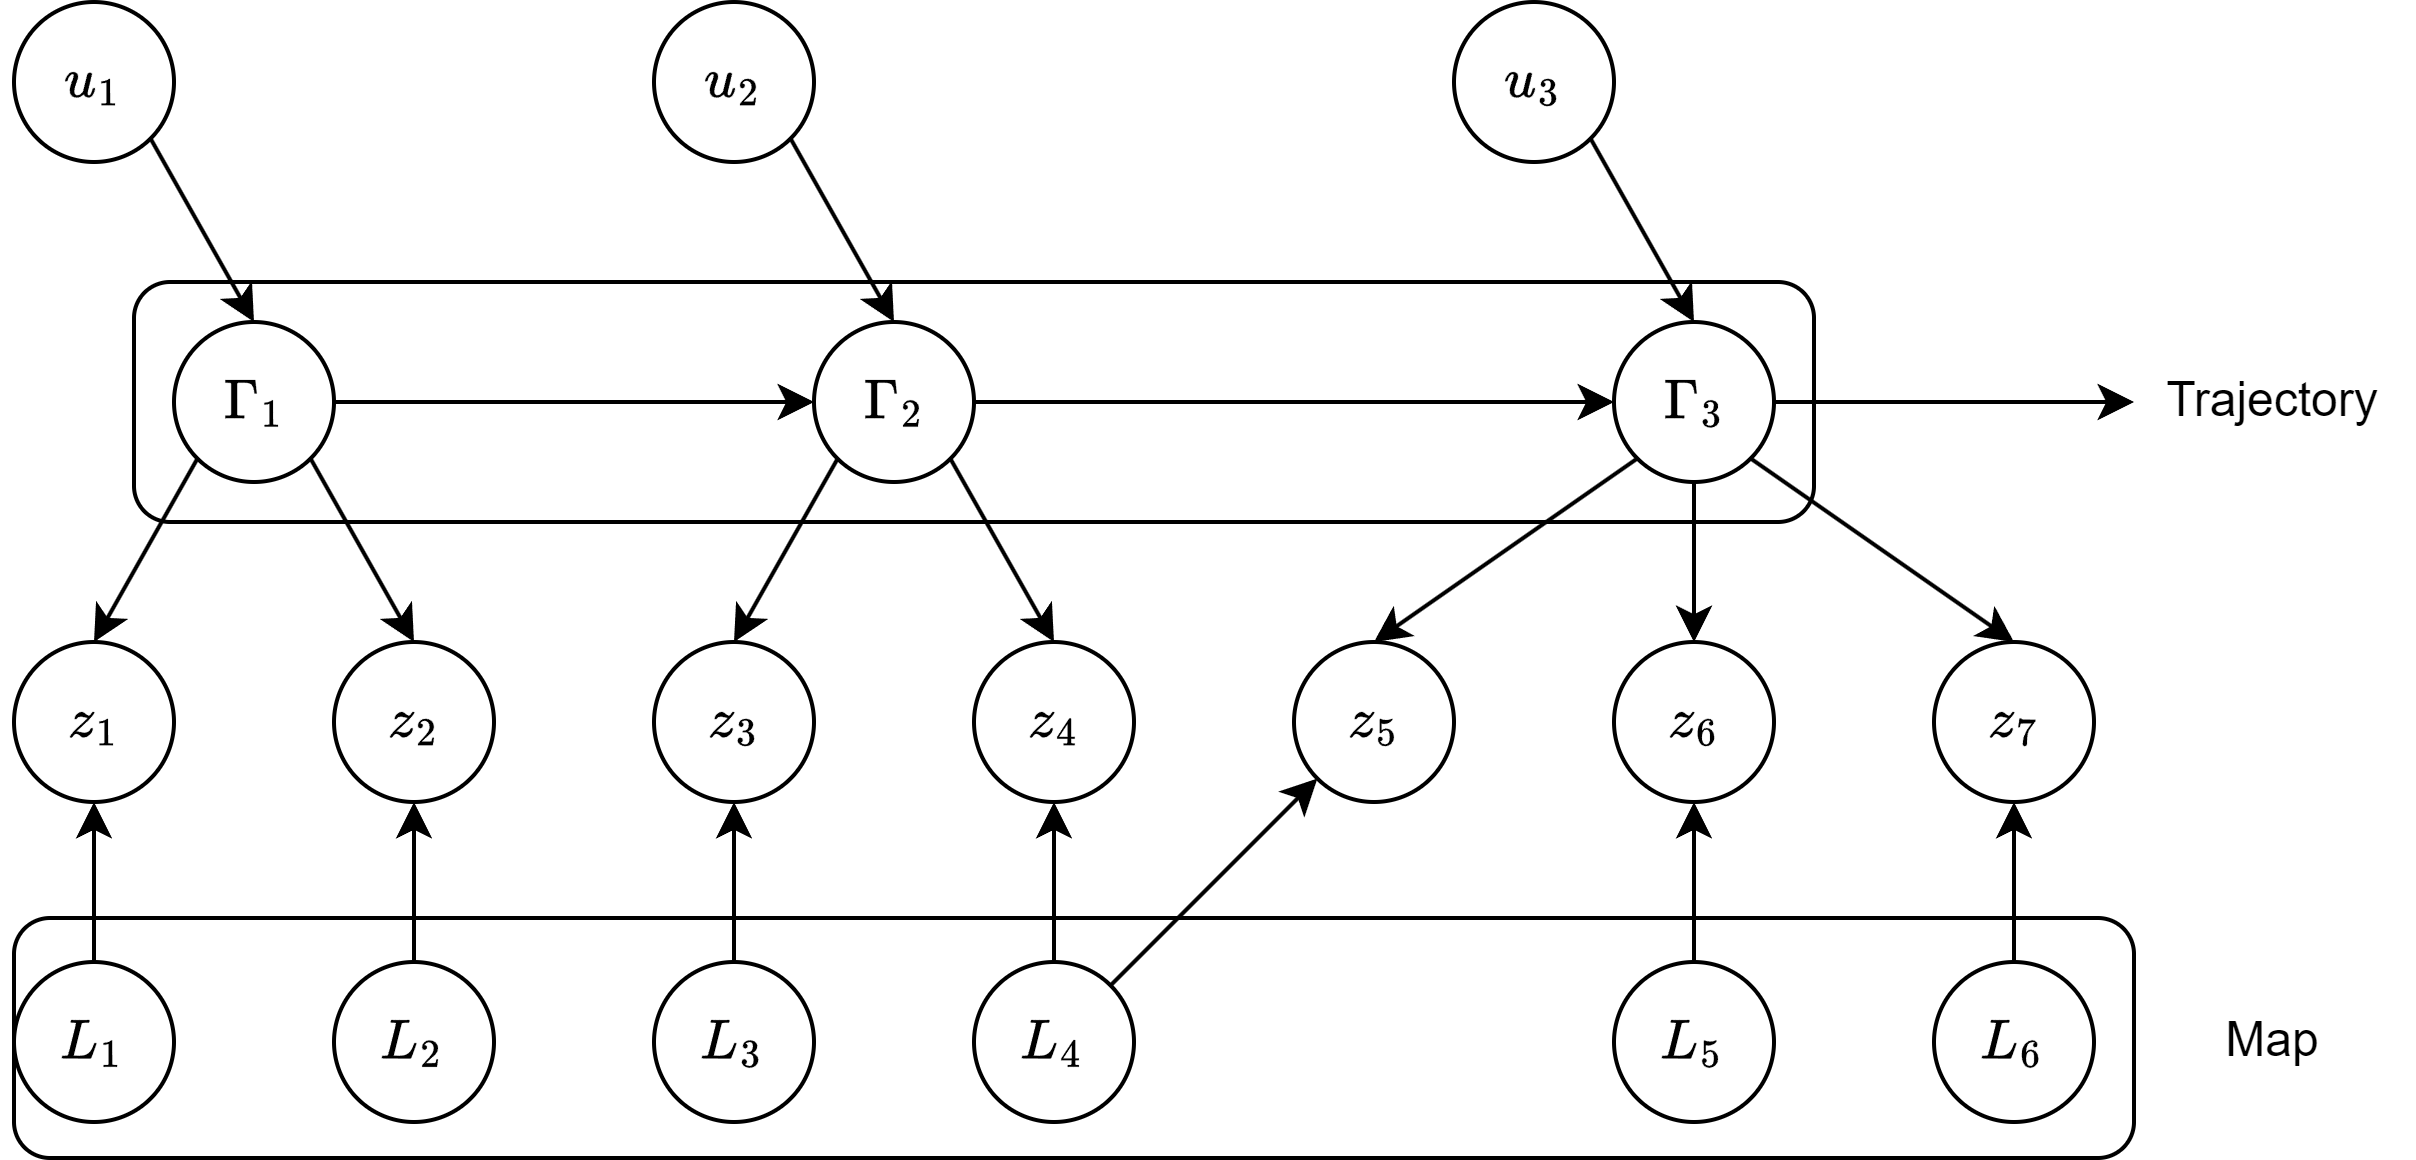
\includegraphics[width=0.75\linewidth]{images/slam.png}
    \caption{Simultaneous localization And Mapping}
\end{figure}
If a complete trajectory isn't necessary, a simplified version known as online SLAM can be used. 
This method provides the entire map and calculates the probability of only the most recent pose based on all measurements and actions: 
\[\text{P}\left(\Gamma_{t},l_1,\dots,l_N|Z_{1:t},U_{1:t}\right)=\int\int\int_{1}^{t-1}\text{P}\left(\Gamma_{1:t},l_1,\dots,l_N|Z_{1:t},U_{1:t}\right)\]
It's important to note that the term pose encompasses not only the position but also the orientation of the robot relative to the environment.

The motion model incorporates all actions $u_1,\dots,u_N$ and their resulting poses $\Gamma_1,\dots,\Gamma_N$ describing how the robot's pose changes through the actuators.

On the other hand, the sensor model involves all poses $\Gamma_1,\dots,\Gamma_N$, all position probabilities $z_1,\dots,z_N$, and the map with landmarks $L_1,\dots,L_N$. 
It defines the probability distribution of a specific measurement given the robot's pose and the positions of the landmarks.